\documentclass[a4paper, 12pt]{article}
\author{\href{mailto:m.robinson@garvan.org.au}{Mark Robinson}  \href{mailto:a.statham@garvan.org.au}{Aaron Statham}  \href{mailto:d.strbenac@garvan.org.au}{Dario Strbenac}}
\usepackage[pdftex]{hyperref}
\usepackage{amsmath}
\usepackage{amssymb}
\usepackage{amscd}
\usepackage{attachfile}
\usepackage{graphicx}
\usepackage[tableposition=top]{caption}
\usepackage{ifthen}
\usepackage[utf8]{inputenc}
\topmargin -.5in
\headheight 0in
\headsep 0in
\oddsidemargin -.5in
\evensidemargin -.5in
\textwidth 176mm
\textheight 245mm

\usepackage{color}
\usepackage{Sweave}

\begin{document}

%\VignetteIndexEntry{Using Repitools for Epigenomic Sequencing Data}

\title{Integrative Analysis of Epigenomic sequencing (and microarray) data with \texttt{Repitools}}
\date{}
\maketitle
\begin{center}
    Last compiled on: \today
\end{center}

\section{Introduction}
\texttt{Repitools} is a package that allows exploratory as well as targeted statistical analysis of absolute and differential binding for ChIP-seq and MeDIP-seq data types, and gives visual summaries in a variety of formats. Some basic quality checking utilities are available for sequencing data. Much of the functionality available is implemented for both tiling microarrays and sequencing data, with very similar function calls for both types of data. \\

In this vignette, we highlight various features within the package.  Further description of the package can be found in the associated Bioinformatics Applications Note\footnote{\href{http://bioinformatics.oxfordjournals.org/content/26/13/1662.abstract}{Repitools: an R package for the analysis of enrichment-based epigenomic data}} as well as in the help documents. \\

To start with, load the \texttt{Repitools} package:

\begin{Schunk}
\begin{Sinput}
> library(Repitools)
\end{Sinput}
\end{Schunk}


\section{Example Datasets}
A small \texttt{GRangesList} of mapped short reads (four samples run on an Illumina Genome Analyser) is included with the package (for example, see \texttt{?binPlots}). This data has been published and is available \href{http://www.ncbi.nlm.nih.gov/geo/query/acc.cgi?acc=GSE24546}{here}. LNCaP is a prostate cancer cell line, and PrEC is a (normal) prostate epithelial cell line.  Here, the ``IP" represents an MBD capture experiment, whereby a population of DNA fragments containing methylated DNA (generally in the CpG context) and ``input" represents fragmented genomic DNA from the same cell lines. \\

Note that \texttt{GRanges} objects of mapped reads from many popular aligners can be created in \textbf{R} using the \texttt{readAligned} function in the \texttt{ShortRead} package, then coerced with \texttt{as(alnRdObj, "GRanges")}. Alternatively, two convenience methods \texttt{BAM2GRanges} and \texttt{BAM2GRangesList} in \texttt{Repitools} could also be used, if the reads were stored on disk in BAM format (this uses the \texttt{scanBam} function from the \texttt{Rsamtools} package). By default, these two methods read in only the uniquely-mapping reads. See the \texttt{ShortRead} package documentation for ideas about how to read other sequencing data into \texttt{GRanges} or \texttt{GRangesList} objects.

\begin{Schunk}
\begin{Sinput}
> library(GenomicRanges)
> load("samplesList.RData")
> class(samples.list)
\end{Sinput}
\begin{Soutput}
[1] "GRangesList"
attr(,"package")
[1] "GenomicRanges"
\end{Soutput}
\begin{Sinput}
> names(samples.list)
\end{Sinput}
\begin{Soutput}
[1] "PrEC input"  "PrEC IP"     "LNCaP input" "LNCaP IP"   
\end{Soutput}
\begin{Sinput}
> elementLengths(samples.list)
\end{Sinput}
\begin{Soutput}
 PrEC input     PrEC IP LNCaP input    LNCaP IP 
   11061279    10008129    19119904    10139044 
\end{Soutput}
\begin{Sinput}
> samples.list[[1]]
\end{Sinput}
\begin{Soutput}
GRanges with 11061279 ranges and 1 elementMetadata value
           seqnames         ranges strand   | pData.alignData.from...notNA...
              <Rle>      <IRanges>  <Rle>   |                       <integer>
       [1]     chr1   [ 248,  283]      +   |                               0
       [2]     chr1   [ 447,  482]      -   |                              16
       [3]     chr1   [ 602,  637]      -   |                              16
       [4]     chr1   [3182, 3217]      +   |                               0
       [5]     chr1   [4783, 4818]      -   |                              16
       [6]     chr1   [6287, 6322]      -   |                              16
       [7]     chr1   [6310, 6345]      +   |                               0
       [8]     chr1   [7340, 7375]      -   |                              16
       [9]     chr1   [9103, 9138]      -   |                              16
       ...      ...            ...    ... ...                             ...
[11061271]     chrM [16531, 16566]      +   |                               0
[11061272]     chrM [16532, 16567]      +   |                               0
[11061273]     chrM [16532, 16567]      -   |                              16
[11061274]     chrM [16533, 16568]      -   |                              16
[11061275]     chrM [16533, 16568]      +   |                               0
[11061276]     chrM [16534, 16569]      -   |                              16
[11061277]     chrM [16535, 16570]      -   |                              16
[11061278]     chrM [16536, 16571]      +   |                               0
[11061279]     chrM [16536, 16571]      -   |                              16

seqlengths
      chr1      chr2      chr3      chr4 ...      chrX      chrY      chrM
 247249719 242951149 199501827 191273063 ... 154913754  57772954     16571
\end{Soutput}
\end{Schunk}


Also, an annotation of genes will be used. The annotation used here is based on one provided from Affymetrix for their Gene 1.0 ST expression arrays\footnote{\href{http://www.affymetrix.com/Auth/analysis/downloads/na27/wtgene/HuGene-1\_0-st-v1.na27.hg18.transcript.csv.zip}{http://www.affymetrix.com/Auth/analysis/downloads/na27/wtgene/HuGene-1\_0-st-v1.na27.hg18.transcript.csv.zip}}. We will relate the epigenomic sequencing data to the Affymetrix gene expression measurements.  Of course, users may wish to make use of the rich functionality available within the \texttt{GenomicFeatures} package.
 
\begin{Schunk}
\begin{Sinput}
> gene.anno <- read.csv("geneAnno.csv", stringsAsFactors = FALSE)
> head(gene.anno)
\end{Sinput}
\begin{Soutput}
     name  chr strand  start    end    symbol
1 7896759 chr1      + 781253 783614 LOC643837
2 7896761 chr1      + 850983 869824    SAMD11
3 7896779 chr1      + 885829 890958    KLHL17
4 7896798 chr1      + 891739 900345   PLEKHN1
5 7896817 chr1      + 938709 939782     ISG15
6 7896822 chr1      + 945365 981355      AGRN
\end{Soutput}
\begin{Sinput}
> dim(gene.anno)
\end{Sinput}
\begin{Soutput}
[1] 24966     6
\end{Soutput}
\end{Schunk}


\noindent Lastly, there is matrix of gene expression changes, with each element related to the corresponding row in the gene annotation table. These values are moderated t-statistics (see the \texttt{limma} package) of background corrected and RMA normalised Affymetrix expression array experiments. The unprocessed array data is available \href{http://www.ncbi.nlm.nih.gov/geo/query/acc.cgi?acc=GSE19726}{here}.

\begin{Schunk}
\begin{Sinput}
> load("expr.RData")
> head(expr)
\end{Sinput}
\begin{Soutput}
            t-stat
7896759  4.1130688
7896761  3.0691214
7896779  0.9724271
7896798 -0.5090460
7896817  2.1949896
7896822 -6.4049774
\end{Soutput}
\begin{Sinput}
> dim(expr)
\end{Sinput}
\begin{Soutput}
[1] 24966     1
\end{Soutput}
\end{Schunk}



\section{Quality Checking}
As mentioned, two of the samples are MBD2 IPs, and two are inputs. Therefore, the IP samples should differ to the inputs in at least two ways. Firstly, they should be more CpG-rich, since we are enriching for methylated DNA, whcih rarely occurs outside of this sequence context. Secondly, DNA methylation tends to occur in peaks since CpG sites are often present in CpG-rich islands.  Conversely, the input samples should be distributed somewhat uniform genome-wide, aside from the usual mappability and GC content biases.\\

We can visualize the (log) frequencies of normalized coverage to get an idea of whether the reads occur in clusters or more dispersed, at least in a relative sense.  For this, we can use \texttt{enrichmentPlot}.  Similarly, we can calculate the CpG density of reads (or reads extended to a certain fragment size) and plot distributions across multiple samples using \texttt{cpgDensityPlot}, as below.

\begin{Schunk}
\begin{Sinput}
> seqinfo(samples.list)
\end{Sinput}
\begin{Soutput}
Seqinfo of length 25
seqnames seqlengths isCircular
chr1      247249719       <NA>
chr2      242951149       <NA>
chr3      199501827       <NA>
chr4      191273063       <NA>
chr5      180857866       <NA>
chr6      170899992       <NA>
chr7      158821424       <NA>
chr8      146274826       <NA>
chr9      140273252       <NA>
...             ...        ...
chr17      78774742       <NA>
chr18      76117153       <NA>
chr19      63811651       <NA>
chr20      62435964       <NA>
chr21      46944323       <NA>
chr22      49691432       <NA>
chrX      154913754       <NA>
chrY       57772954       <NA>
chrM          16571       <NA>
\end{Soutput}
\begin{Sinput}
> enrichmentPlot(samples.list, seq.len = 300, cols = c("black", 
+     "green", "orange", "red"), xlim = c(0, 10), lwd = 2)
\end{Sinput}
\end{Schunk}
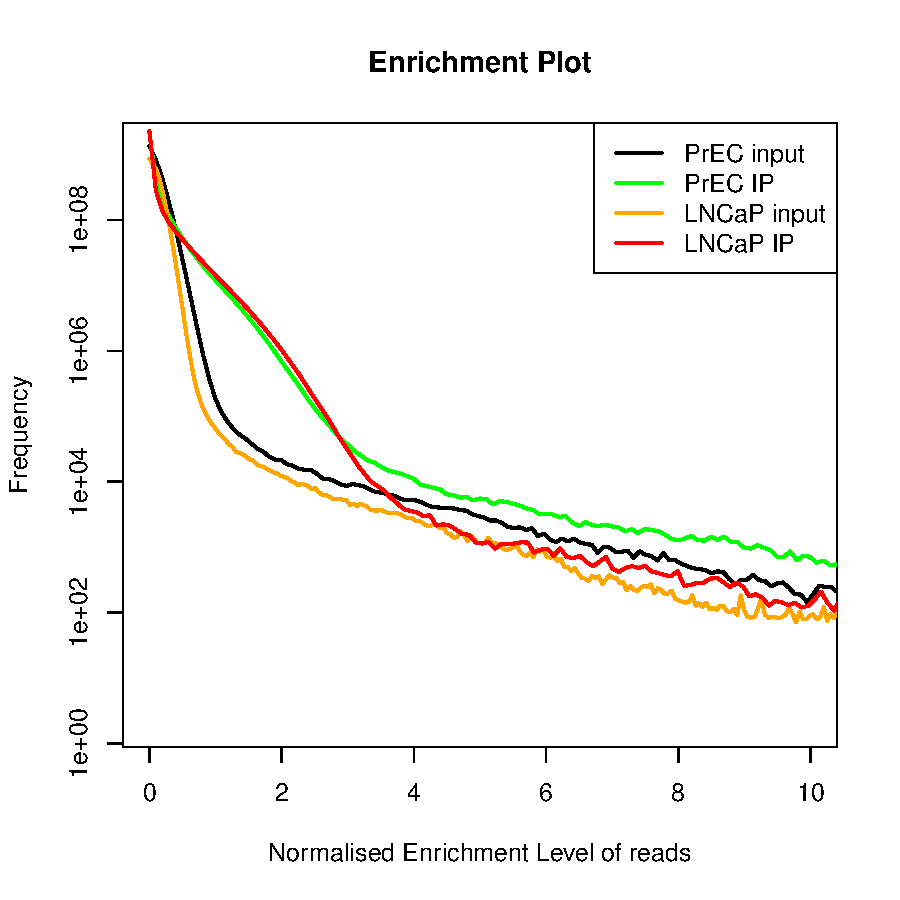
\includegraphics{enrPlot-enrPlot}


\noindent The code makes use of the SeqInfo annotation of \texttt{samples.list} to retrieve the maximum base of chromosomes.  Normalization scales coverage value to ``reads per 10 million". The argument \texttt{seq.len=300} is passed in as the length to extend reads to, since that is approximately the real length of the fragments sequenced in this experiment. As expected, many more bases in the IP samples have high read coverages. \\
\ \\
An alternative comparative visualization, which is somewhat specific to methylated DNA enrichment experiments, is a summary of the distribution of CpG density among reads/fragments:

\begin{Schunk}
\begin{Sinput}
> library(BSgenome.Hsapiens.UCSC.hg18)
> cpgDensityPlot(samples.list, organism = Hsapiens, w.function = "none", 
+     seq.len = 300, cols = c("black", "green", "orange", "red"), 
+     xlim = c(0, 30), lwd = 2)
\end{Sinput}
\end{Schunk}
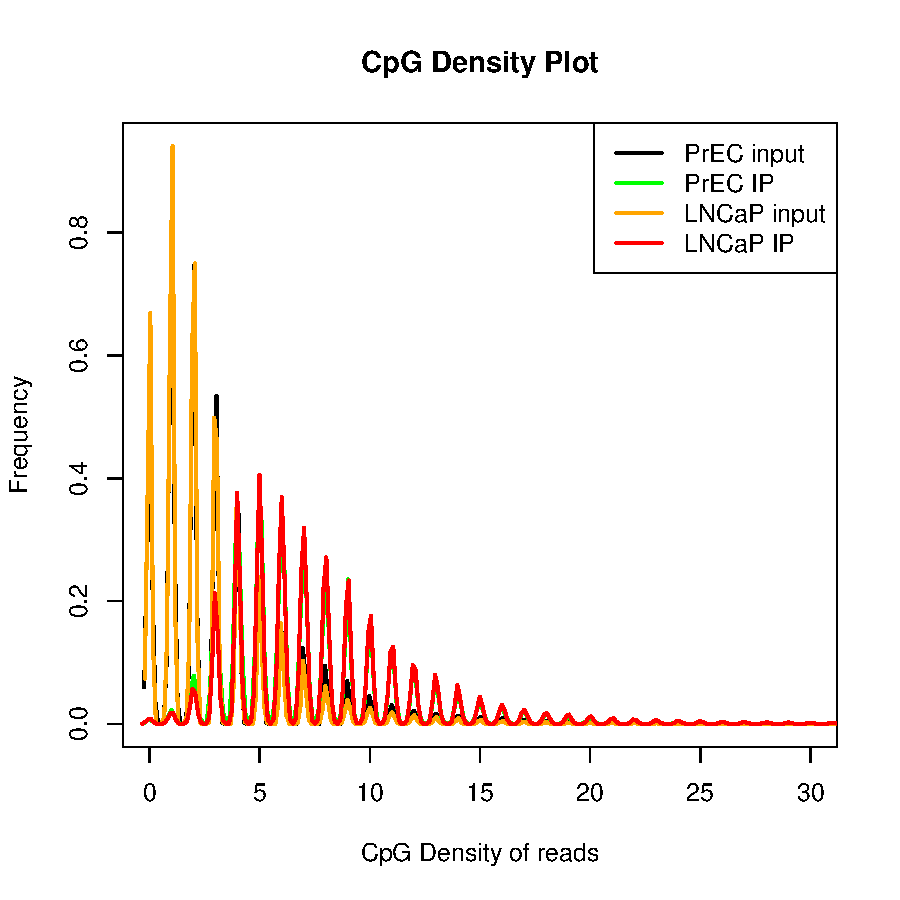
\includegraphics{cpgPlot-cpgPlot}


\noindent The full genome sequence of the organism is required so that the (here, 300 base) DNA sequence can be fetched. In this example, the \texttt{BSgenome} package of the hg18 assembly for human is used (many other BSgenome objects for other organisms are available from Bioconductor). The \texttt{w.function} parameter allows the count of CpGs to be weighted. In this example, raw counts are used.
\ \\ \ \\
Notice that at lower CpG densities, the two input samples have a higher frequency of reads than the two IP samples. At higher CpG densities, this trend is reversed. This suggests that the enrichment of methylated CpGs has worked.
\ \\ \ \\
% \noindent For more general sequencing quality checking, the FastQC \footnote{\href{http://www.bioinformatics.bbsrc.ac.uk/projects/fastqc/}{http://www.bioinformatics.bbsrc.ac.uk/projects/fastqc/}} Java application has been gaining popularity due to its speed and variety of results. A container class, \texttt{FastQC}, accessors, and the method \texttt{readFastQC} for reading in the raw Java program text file output and creating a FastQC \textbf{R} object, have been made to provide a framework for the fast development of quality control report generating pipelines. Higher level container classes with accessor methods are \texttt{SequenceQC}, which groups \texttt{FastQC} objects for the aligned and unaligned reads of a single sample together, and \texttt{SequenceQCSet} which is a collection of \texttt{SequenceQC} objects, perhaps of multiple sequencing samples within the same experimental run.
% \\ \\
% An example of turning a set of FastQC text output files of the DNA methylation read data into a quality report PDF is demonstrated next.

% <<label=QCreport>>=
% load("QCset.RData")
% summary(QCset)

% pdf("QCreport.pdf", height = 8, width = 12)
% genQC(QCset, "DNA Methylation Experiment")
% dev.off()
% @

% Click here to see the report. \attachfile[icon=Paperclip]{QCreport.pdf}
% \\ \\
% When looking at the base distributions of the inputs, for either all of the reads, or the aligned subset, it can be seen that the frequency of A or T is always more than the G or C frequency. This mirrors the background distribution of the human genome. In the IP samples, the G or C frequency has risen, and the A or T has dropped, as would be expected when enriching for GC rich DNA methylated sequences.
% \\ \\
% This mismatches-by-cycles plots show that the IP samples tend to have a bias of G being called as T, and this is independent of the sequencing cycle. PrEC input has a tendency to miscall T as G more often than any other error, no matter the cycle.

\section{Analyses}

\subsection{Statistics of Differential Enrichment}
The \texttt{blocksStats} function is a convenient way to do statistical tests of differential enrichment between two experimental conditions, using counts in regions of interest. The windows can be relative to some genomic landmarks, like transcription start sites (TSSs), and their size can be specified with the \texttt{up} and \texttt{down} parameters. If \texttt{up} and \texttt{down} are not provided, then windows are defined by start and end coordinates. The function leverages \texttt{edgeR}'s count modelling and its adaptation of Fisher's exact test for assessing differential enrichment.  The procedure also uses Bioconductor's facilities (i.e. \texttt{countOverlaps}) for counting mapped read in regions of the genome.

\begin{Schunk}
\begin{Sinput}
> design.matrix <- matrix(c(0, -1, 0, 1), dimnames = list(names(samples.list), 
+     "C-N"))
> design.matrix
\end{Sinput}
\begin{Soutput}
            C-N
PrEC input    0
PrEC IP      -1
LNCaP input   0
LNCaP IP      1
\end{Soutput}
\begin{Sinput}
> stats <- blocksStats(samples.list, gene.anno, up = 2000, down = 0, 
+     seq.len = 300, design = design.matrix)
\end{Sinput}
\begin{Soutput}
Comparison of groups:  1 - -1 
\end{Soutput}
\begin{Sinput}
> stats <- stats[order(stats$`adj.p.vals_C-N`), ]
> head(stats)
\end{Sinput}
\begin{Soutput}
          chr     start       end width strand    name symbol PrEC input
8019804 chr18     99064    112217 13154      + 8019804  ROCK1        600
8015798 chr17  38802738  38821439 18702      - 8015798    ---         87
7904879  chr1 145017918 145018085   168      + 7904879    ---         21
7908529  chr1 196148257 196165896 17640      + 7908529   LHX9         16
8115391  chr5 153834725 153838017  3293      - 8115391  HAND1          8
7976073 chr14  85066240  85164023 97784      + 7976073  FLRT2         17
        PrEC IP LNCaP input LNCaP IP PrEC IP_pseudo LNCaP IP_pseudo logConc_C-N
8019804     397         686       58   3.995887e+02        57.62379   -16.01856
8015798      56          64      314   5.636562e+01       311.96569   -16.21306
7904879      13          28      153   1.308530e+01       152.00848   -17.78513
7908529       3          13      112   3.020114e+00       111.27404   -19.06788
8115391       4          28       95   4.026631e+00        94.38415   -18.97912
7976073       0          20       69   1.435022e-11        68.55255   -33.59047
        logFC_C-N  p.value_C-N adj.p.vals_C-N
8019804 -2.793764 9.642793e-36   2.407420e-31
8015798  2.468516 3.662695e-24   4.572142e-20
7904879  3.538199 3.672510e-18   3.056262e-14
7908529  5.203643 7.401219e-18   4.619471e-14
8115391  4.551106 2.875722e-14   1.435905e-10
7976073 32.851160 1.911561e-13   7.954003e-10
\end{Soutput}
\end{Schunk}


\noindent Note that this is {\em not} a real design matrix (in a statistical sense), it is simply a way of specifying the two experiment conditions to compare (they must be 1 and -1). \\

\noindent The example above calculates statistics on regions that start 2000 bases upstream of the TSS and finish at the TSS, after the reads have been extended to being 300 bases. A coverage plot from UCSC browser illustrates the best found region.  For the output table, the read counts are scaled as if there were 10 million reads covering the regions of interest. \\

\noindent Note that this procedure only works for simple 2-group comparisons.  Using this strategy for more complicated designs requires manually creating the count tables (see \texttt{annotationCounts} below) and calling the GLM-based procedures (e.g. using real design matrices) within \texttt{edgeR}. \\


\begin{figure}[!h]
    \begin{center}
        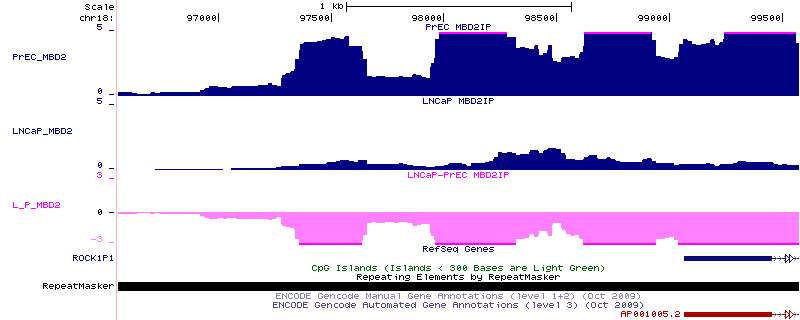
\includegraphics{rock1.png}
    \end{center}
\end{figure}

This differential enrichment strategy can be used on bins covering the entire genome.  The \texttt{genomeBlocks} function can be used to generate windows along the genome.


\subsection{Domains of Concordant Change}

Another analysis of interest is the detection of {\em regions} where changes in expression (or an epigenetic mark, etc.) occur on a particular chromosome. The function \texttt{findClusters} addresses this need. The method of determining clusters requires a search through the column of scores (e.g. t-statistics) for a persistent change.  Significance of clusters is determined by randomization.  The order of the statistics is permuted a large number of times and the number of clusters found in the true statistics column and the permuted statistics columns is counted, ranging from a loose cutoff to a tight cutoff.  A cutoff is chosen to control the user-specified FDR. Importantly, the table must be pre-sorted in positional order. This allows the user to use whatever definition of position they want.  Note that the distance between features is not taken into account in this implementation.

\begin{Schunk}
\begin{Sinput}
> stats.table <- cbind(gene.anno, expr)
> stats.table$pos <- ifelse(stats.table$strand == "+", stats.table$start, 
+     stats.table$end)
> pos.order <- order(stats.table$chr, stats.table$pos)
> stats.table <- stats.table[pos.order, ]
> stats.clustered <- findClusters(stats.table, score.col = 7, w.size = 5, 
+     n.med = 2, n.consec = 3, cut.samps = seq(-2, -10, -2), maxFDR = 0.05, 
+     trend = "down", n.perm = 10)
> cluster.1 <- which(stats.clustered$cluster == 1)
> stats.clustered[cluster.1, ]
\end{Sinput}
\begin{Soutput}
           name  chr strand    start      end  symbol      t-stat      pos
7914667 7914667 chr1      - 33829993 33947691   CSMD2  -0.8496609 33947691
7899898 7899898 chr1      + 34102217 34102979   HMGB4  -0.2014024 34102217
7899905 7899905 chr1      + 34102217 34102979   HMGB4  -0.1829972 34102217
7914748 7914748 chr1      - 34251727 34252405     ---  -0.3865665 34252405
7899911 7899911 chr1      + 34405070 34457319 C1orf94  -0.9322332 34405070
7899921 7899921 chr1      + 34993307 34996699    GJB5 -16.4867896 34993307
7899927 7899927 chr1      + 34999364 35000515    GJB4  -8.2965082 34999364
7899932 7899932 chr1      + 35019376 35024552    GJB3 -11.7589771 35019376
7899939 7899939 chr1      + 35031185 35033935    GJA4  -0.2142715 35031185
        cluster
7914667       1
7899898       1
7899905       1
7914748       1
7899911       1
7899921       1
7899927       1
7899932       1
7899939       1
\end{Soutput}
\end{Schunk}


\noindent In this example, a running window of 5 consecutive genes is calculated along each chromosome; the median value of those 5 genes is assigned to the middle gene. If, in the 5-gene window, there are at least 2 genes that have an assigned median above the cutoff being used (cutoffs of -2, -4, -6, -8, and -10 are tried), then those genes are candidate cluster-generating genes. Starting from a candidate gene, and working outwards until encountering a positive t-statistic, if a consecutive run of at least 3 genes with t-statistic being negative could be made, then this forms a cluster. The default estimated FDR of 0.05 is used.

\subsection{Finding enriched regions in a single sample}
Repitools contains an implementation of \texttt{ChromaBlocks} (described in \href{http://www.ncbi.nlm.nih.gov/pubmed/20452322}{Hawkins RD et al}), designed to discover regions of the genome which are enriched for epigenetic marks, such as H3K27me3.  Briefly, ChromaBlocks counts the number of sequencing reads aligned to adjacent bins in the genome in both Immunoprecipitated and Input samples, determines which bins exceed a cutoff for IP-Input enrichment (either specified or set at a supplied FDR by permutation) and returns regions of the genome where multiple adjacent bins are enriched.

\noindent Data from the Human Reference Epigenome Mapping Project is used to demonstrate \texttt{ChromaBlocks}. The data was downloaded from \href{http://www.ncbi.nlm.nih.gov/geo/query/acc.cgi?acc=GSE16256}{here}. Samples \href{http://www.ncbi.nlm.nih.gov/geo/query/acc.cgi?acc=GSM466734}{GSM466734}, \href{http://www.ncbi.nlm.nih.gov/geo/query/acc.cgi?acc=GSM466737}{GSM466737}, \href{http://www.ncbi.nlm.nih.gov/geo/query/acc.cgi?acc=GSM466739}{GSM466739}, and \href{http://www.ncbi.nlm.nih.gov/projects/geo/query/acc.cgi?acc=GSM450270}{GSM450270} are used here.

\begin{Schunk}
\begin{Sinput}
> load("H1samples.RData")
> class(H1samples)
\end{Sinput}
\begin{Soutput}
[1] "GRangesList"
attr(,"package")
[1] "GenomicRanges"
\end{Soutput}
\begin{Sinput}
> names(H1samples)
\end{Sinput}
\begin{Soutput}
[1] "H3K4me1"  "H3K27me3" "H3K36me3" "Input"   
\end{Soutput}
\begin{Sinput}
> elementLengths(H1samples)
\end{Sinput}
\begin{Soutput}
 H3K4me1 H3K27me3 H3K36me3    Input 
 1201402  8673675  4151895 15289957 
\end{Soutput}
\begin{Sinput}
> H3K27me3.blocks <- ChromaBlocks(rs.ip = H1samples["H3K27me3"], 
+     rs.input = H1samples["Input"], organism = Hsapiens, chrs = "chr20", 
+     preset = "small", seq.len = 300)
\end{Sinput}
\begin{Soutput}
Permutation 1.
Permutation 2.
Permutation 3.
Permutation 4.
Permutation 5.
Testing positive regions.
Using cutoff of 2.337163 for a FDR of 0.01 
.
\end{Soutput}
\end{Schunk}


\texttt{ChromaBlocks} returns a \texttt{ChromaResults} object, from which an \texttt{IRangesList} of the regions determined to be enriched can be retrieved using the \texttt{regions} method.

\begin{Schunk}
\begin{Sinput}
> H3K27me3.blocks
\end{Sinput}
\begin{Soutput}
Object of class 'ChromaResults'.
1400 regions found with using a cutoff of 2.337163 
\end{Soutput}
\begin{Sinput}
> regions(H3K27me3.blocks)
\end{Sinput}
\begin{Soutput}
SimpleRangesList of length 1
$chr20
IRanges of length 1400
          start      end width
[1]       60150    61550  1401
[2]      189750   191050  1301
[3]      228950   236350  7401
[4]      237050   243050  6001
[5]      243450   245550  2101
[6]      245850   248250  2401
[7]      259250   260950  1701
[8]      275950   277950  2001
[9]      279350   281050  1701
...         ...      ...   ...
[1392] 62185050 62186750  1701
[1393] 62204850 62206750  1901
[1394] 62272950 62274750  1801
[1395] 62282050 62285250  3201
[1396] 62362950 62364450  1501
[1397] 62367750 62371150  3401
[1398] 62404450 62405650  1201
[1399] 62407650 62409450  1801
[1400] 62426850 62428550  1701
\end{Soutput}
\end{Schunk}


\section{Visualisations}

The visualisations in the following two subsections manipulate matrices of scores (such as coverages or intensities) in some way, such as clustering them, or summarising them by some defined grouping. The common interface for creating matrices of scores at regular distances from a reference point, such a TSS, is the \texttt{featureScores} function. The following example samples smoothed coverages between 5000 bases upstream of gene TSSs, and 1000 bases downstream of the TSS, at 1000 base intervals, in the PrEC and LNCaP immunoprecipitated samples. The scores are then subtracted from each other.

\begin{Schunk}
\begin{Sinput}
> prostateCvgs <- featureScores(samples.list[c("PrEC IP", "LNCaP IP")], 
+     gene.anno, up = 5000, down = 1000, freq = 1000, s.width = 500)
> prostateCvgs
\end{Sinput}
\begin{Soutput}
An object of class 'ScoresList'.
Tables: PrEC IP, LNCaP IP.
Features:
GRanges with 24966 ranges and 2 elementMetadata values
        seqnames               ranges strand   |      name      symbol
           <Rle>            <IRanges>  <Rle>   | <integer> <character>
    [1]     chr1   [ 781253,  783614]      +   |   7896759   LOC643837
    [2]     chr1   [ 850983,  869824]      +   |   7896761      SAMD11
    [3]     chr1   [ 885829,  890958]      +   |   7896779      KLHL17
    [4]     chr1   [ 891739,  900345]      +   |   7896798     PLEKHN1
    [5]     chr1   [ 938709,  939782]      +   |   7896817       ISG15
    [6]     chr1   [ 945365,  981355]      +   |   7896822        AGRN
    [7]     chr1   [1092346, 1092441]      +   |   7896859         ---
    [8]     chr1   [1093105, 1093195]      +   |   7896861         ---
    [9]     chr1   [1094247, 1094330]      +   |   7896863         ---
    ...      ...                  ...    ... ...       ...         ...
[24958]     chrY [19611913, 19614093]      -   |   8177222        CD24
[24959]     chrY [19640262, 19640361]      -   |   8177227         ---
[24960]     chrY [20076704, 20124427]      -   |   8177229      BCORL2
[24961]     chrY [20326698, 20366197]      -   |   8177232     JARID1D
[24962]     chrY [21036941, 21090502]      -   |   8177261      TTTY10
[24963]     chrY [21954227, 21957634]      -   |   8177273         ---
[24964]     chrY [22001970, 22008519]      -   |   8177280         ---
[24965]     chrY [22154873, 22165940]      -   |   8177282      TTTY13
[24966]     chrY [22852332, 22854411]      -   |   8177344       TTTY5

seqlengths
  chr1 chr10 chr11 chr12 chr13 chr14 ...  chr6  chr7  chr8  chr9  chrX  chrY
    NA    NA    NA    NA    NA    NA ...    NA    NA    NA    NA    NA    NA
Region: 5000 bases up to 1000 bases down.
Smoothing: 500, 500 bases.
Sampling : 1000 bases.
\end{Soutput}
\begin{Sinput}
> prostateCvgs@scores <- list(tables(prostateCvgs)[[2]] - tables(prostateCvgs)[[1]])
> names(prostateCvgs) <- "LNCaP - PrEC"
\end{Sinput}
\end{Schunk}


This object will be used in the next few visualisation functions.

\subsection{Integrative analysis of epigenetics and gene expression}
\noindent Epigenomic data is often gathered with other data, such as gene expression. It may be of interest to see the profile of epigenetic enrichment at a variety of distances from TSSs, stratified by gene expression level. The \texttt{binPlots} function is a convenient way to look at these interactions.

\begin{Schunk}
\begin{Sinput}
> binPlots(prostateCvgs, ordering = expr, ord.label = "Cancer-Normal t-stat", 
+     plot.type = "heatmap", n.bins = 50)
\end{Sinput}
\end{Schunk}
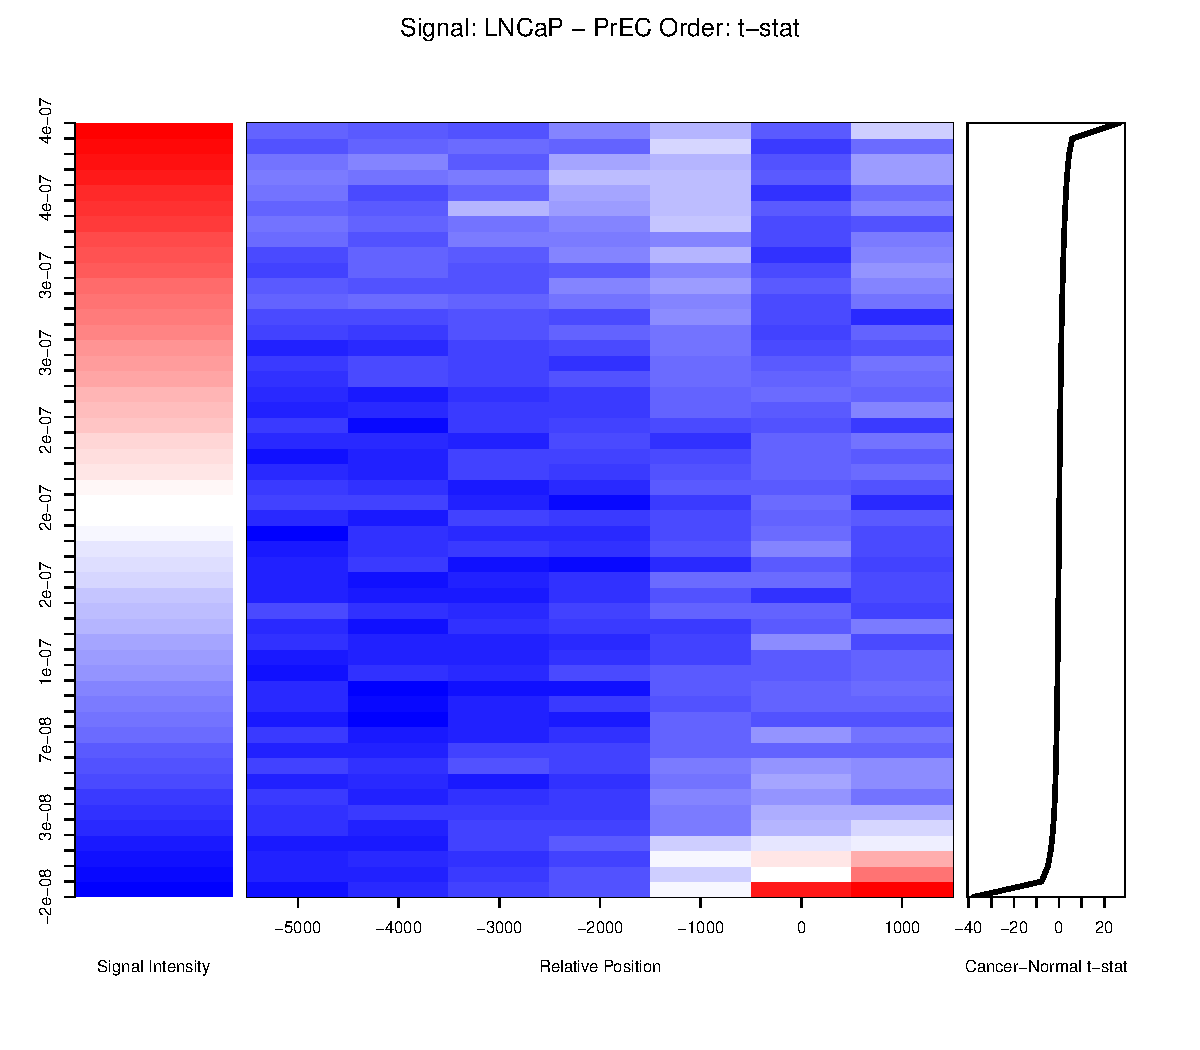
\includegraphics{binPlotsHeatmap-binPlotsHeatmap}


\noindent Enrichment levels (here, differential enrichment) are split into bins based on the moderated t-statistics for change in expression.  Signal for (differential) enrichment is averaged over genes in the bin and plotted as a heatmap.  As expected, the genes that are silenced in cancer exhibit higher levels of DNA methylation around their TSS, compared to normal cells.  This visualization can be represented as a lineplot, by setting \texttt{plot.type= "line"} (see below). \\

\begin{Schunk}
\begin{Sinput}
> binPlots(prostateCvgs, ordering = expr, ord.label = "Cancer-Normal t-stat", 
+     plot.type = "line", n.bins = 10)
\end{Sinput}
\end{Schunk}
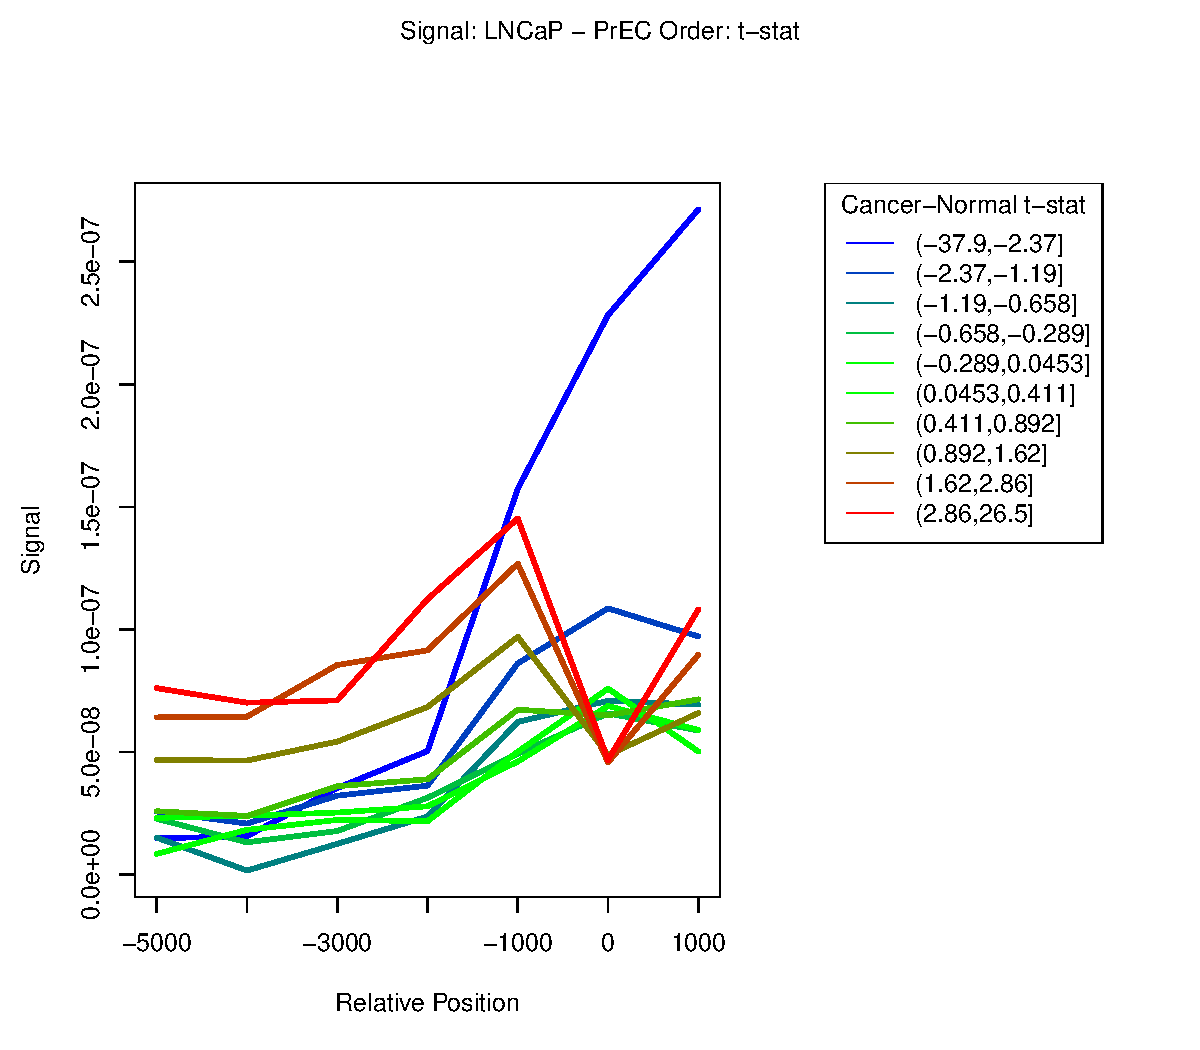
\includegraphics{binPlotsLine-binPlotsLine}


This strategy is useful for determining the location (e.g. relative to TSS) signal most often occurs relative to expression and can be coupled to ranked gene expression levels, instead of differential expression.  These determined regions of interest relative to TSS can then be used in targeted analyses (e.g. \texttt{blocksStats}, see above).

\subsection{Gene Set Enrichment}

Sets of genes (e.g. genes disrupted in a certain type of cancer, or differentially expressed between experimental conditions) are ever-present in genomics research.  For such genes of interest, the profile of intensities or counts can be plotted versus the profile of randomly selected gene lists using the \texttt{profilePlots} function. In the following example, the DNA methylation profile of genes silenced in cancer is significantly different to random sets of genes.

\begin{Schunk}
\begin{Sinput}
> which.loss <- which(expr < -3)
> profilePlots(prostateCvgs, gene.list = list(`Downregulated Genes` = which.loss), 
+     cols = "red")
\end{Sinput}
\end{Schunk}
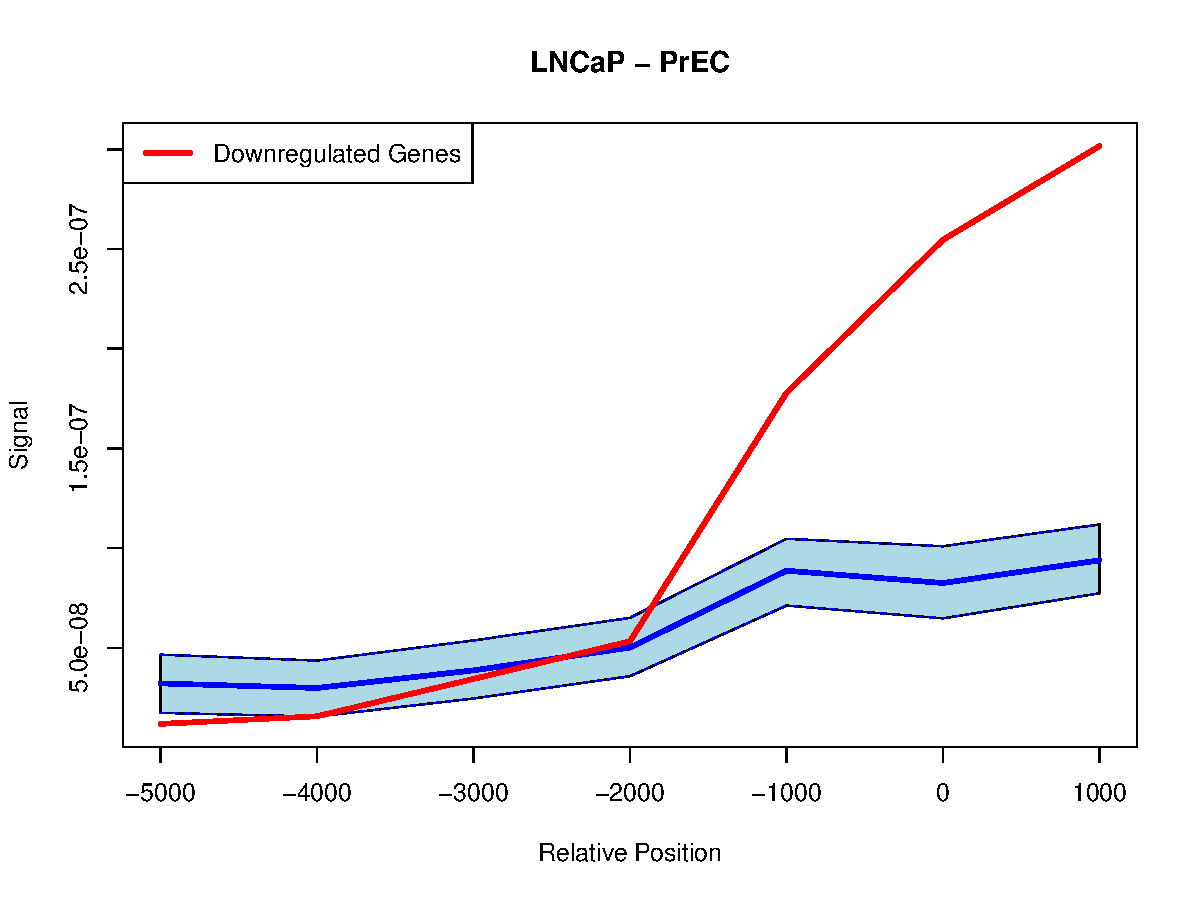
\includegraphics{profPlots-profPlots}


\noindent The blue region forms the ``null" distribution that was created by sampling random gene lists of the same size as the user-specified gene list a number of times, as set by the \texttt{nSamples} parameter. By default, the null region is a between the 0.025 and 0.975 quantiles of the null distribution. In this example, it appears that the genes silenced in cancer have a significant gain of methylation 2000 bases either side of the TSSs, in comparison to random sets of other genes.
\ \\ \ \\

\subsection{Clustering epigenomic signals}

\texttt{clusterPlots} is another way to look at read depth at regular positions around a feature (e.g. TSS). The first step is to use \texttt{featureScores} to get the coverage tables, which essentially gives a list of coverage tables for the samples used. \texttt{clusterPlots} is then called, which does k-means clustering, or if the user wants to use their own clustering algorithm, the cluster ID of each feature can be passed in. In any case, the features are grouped by their cluster memberships and plotted as either a heatmap with one row for every feature, or a set of lineplots showing the average coverage of all features belonging to each cluster. If gene expression data is also available, it can be plotted alongside the heatmaps.

\begin{Schunk}
\begin{Sinput}
> cvgs <- featureScores(H1samples[1:3], gene.anno, up = 5000, down = 2000, 
+     dist = "base", freq = 200, s.width = 500)
\end{Sinput}
\end{Schunk}


\begin{Schunk}
\begin{Sinput}
> cp <- clusterPlots(cvgs, scale = function(x) sqrt(x), plot.type = "heatmap", 
+     t.name = "H1 Cells", n.clusters = 10)
\end{Sinput}
\end{Schunk}

\begin{Schunk}
\begin{Soutput}
pdf 
  2 
\end{Soutput}
\end{Schunk}


Here, we have scaled the signal using the square root transformation.  If you don't specify this, no scaling is done.

\begin{figure}[!h]
    \begin{center}
        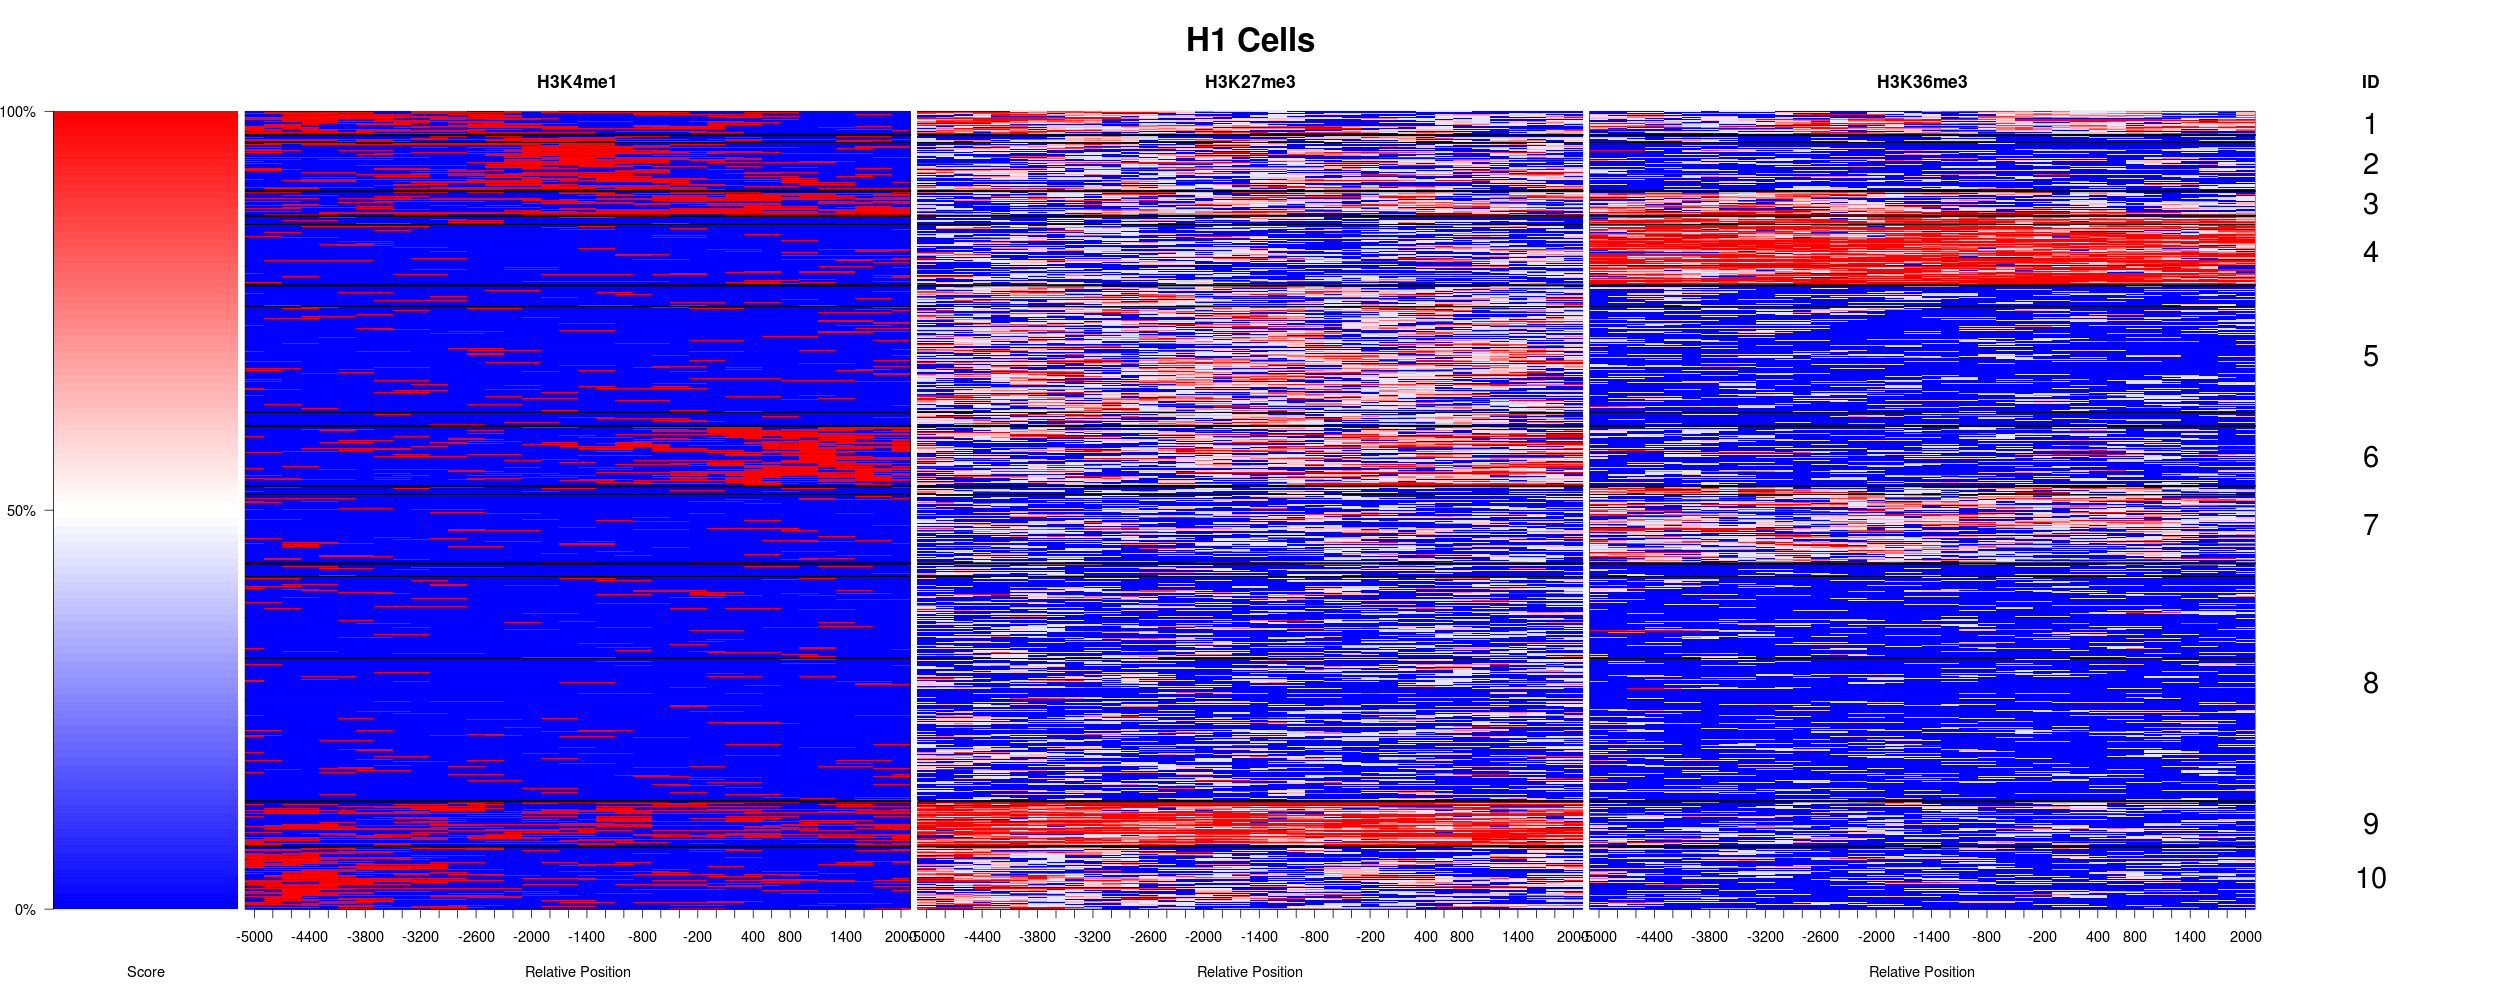
\includegraphics[height=0.48\textheight, width = 1.1\textwidth]{clusterPlot.png}
    \end{center}
\end{figure}

Note that we have saved the output of \texttt{clusterPlots} (a \texttt{ClusteredCoverageList} object), which can be plotted in alternative ways, such as line plots: 

\begin{Schunk}
\begin{Sinput}
> table(clusters(cp))
\end{Sinput}
\begin{Soutput}
   1    2    3    4    5    6    7    8    9   10 
 742 1754  773 2176 4400 1883 2419 7442 1414 1963 
\end{Soutput}
\begin{Sinput}
> clusterPlots(cp, plot.type = "line", t.name = "H1 Cells")
\end{Sinput}
\end{Schunk}
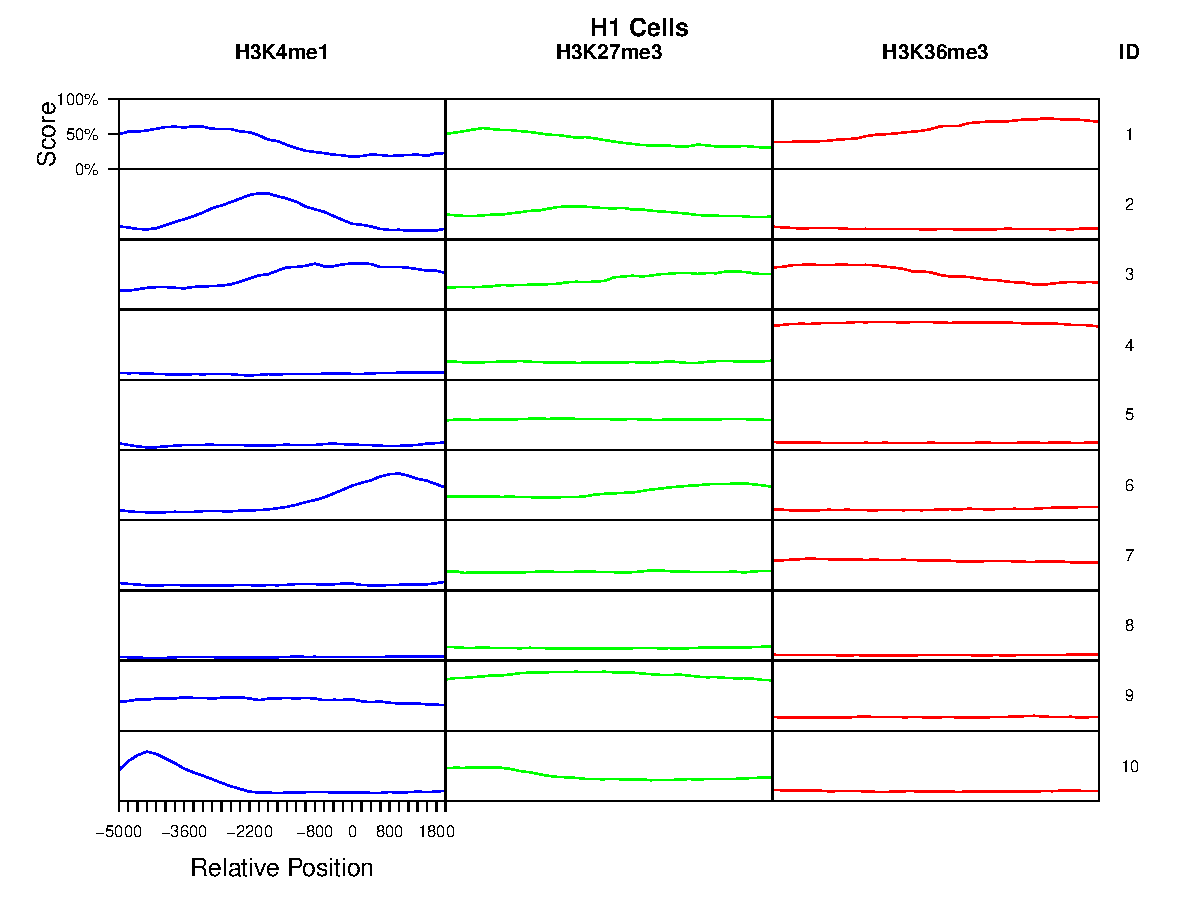
\includegraphics{clusterPlotsLine-cluPlots3}


Also, this allows users to do there own clustering and use \texttt{clusterPlots} for the plotting, or to extract the cluster identifiers for downstream analyses (e.g. functional category analysis).  Furthermore, in addition to specifying a vector of expression values and plotting it alongside the clustered epigenetic signal, users can give an additional vector in the \texttt{sort.data} argument to sort on within a cluster (e.g. gene length, CpG density, etc.).

\section{Utility Functions}

The function described in this section perform useful tasks that are commonly made with epigenetic data.
\subsection{Windows and Counts}
Often, it is required to create a set of windows covering the entire genome, for some analysis. The function \texttt{genomeBlocks} does this.

\begin{Schunk}
\begin{Sinput}
> library(BSgenome.Hsapiens.UCSC.hg18)
> genomeBlocks(Hsapiens, chrs = 1:25, width = 5000)
\end{Sinput}
\begin{Soutput}
GRanges with 616087 ranges and 0 elementMetadata values
         seqnames               ranges strand   |
            <Rle>            <IRanges>  <Rle>   |
     [1]     chr1       [    1,  5000]      *   |
     [2]     chr1       [ 5001, 10000]      *   |
     [3]     chr1       [10001, 15000]      *   |
     [4]     chr1       [15001, 20000]      *   |
     [5]     chr1       [20001, 25000]      *   |
     [6]     chr1       [25001, 30000]      *   |
     [7]     chr1       [30001, 35000]      *   |
     [8]     chr1       [35001, 40000]      *   |
     [9]     chr1       [40001, 45000]      *   |
     ...      ...                  ...    ... ...
[616079]     chrY [57745001, 57750000]      *   |
[616080]     chrY [57750001, 57755000]      *   |
[616081]     chrY [57755001, 57760000]      *   |
[616082]     chrY [57760001, 57765000]      *   |
[616083]     chrY [57765001, 57770000]      *   |
[616084]     chrY [57770001, 57772954]      *   |
[616085]     chrM [       1,     5000]      *   |
[616086]     chrM [    5001,    10000]      *   |
[616087]     chrM [   10001,    15000]      *   |

seqlengths
  chr1  chr2  chr3  chr4  chr5  chr6 ... chr20 chr21 chr22  chrX  chrY  chrM
    NA    NA    NA    NA    NA    NA ...    NA    NA    NA    NA    NA    NA
\end{Soutput}
\end{Schunk}


\noindent This example makes a \texttt{GRanges} object of 5 kb windows along all human chromosomes.
\ \\ \ \\
\texttt{annotationCounts} is useful to tally the counts of reads surrounding some set of genomic landmarks. \texttt{annotationBlocksCounts} is the analogous function for counting in user-specified regions of the genome.

\begin{Schunk}
\begin{Sinput}
> annotationCounts(samples.list, head(gene.anno, 10), up = 2000, 
+     down = 500, seq.len = 300)
\end{Sinput}
\begin{Soutput}
        PrEC input PrEC IP LNCaP input LNCaP IP
7896759         25      35          29       69
7896761         10       2           8       36
7896779         11      15          10       14
7896798         19      61          15       83
7896817         20      41          22       46
7896822         11      17           8       28
7896859         24      35           8       70
7896861         21      57           6       78
7896863         18      85           8       85
7896865         22      92          18       90
\end{Soutput}
\end{Schunk}

	
\noindent This example counts reads that fall within 2000 bases upstream and 500 bases downstream of (the first ten) TSSs in the gene annotation table.  Reads are extended to 300 bases.

\subsection{Characteristics of the DNA sequence}
It would be useful to know when seeing a lack of reads in some windows, if the mappability of the window is the cause. Some regions of the genome have low complexity sequence, where reads are unlikely to map uniquely to. The function \texttt{mappabilityCalc} calculates the percentage of each region that can be mapped to by reads generated from the experiment. It operates on a user-created \texttt{BSgenome} object of a masked genome sequence. The definition of which bases are mappable and which are not depends on the read length of the sequencing technology used. Therefore, there is no one masked \texttt{BSgenome} object that can be used by all users. Note that by masking, we mean replacing the unmappable reference sequence bases by `N', not creating a built-in mask.

\begin{Schunk}
\begin{Sinput}
> library(BSgenome.Hsapiens36bp.UCSC.hg18mappability)
> locations <- data.frame(chr = c("chr4", "chr9"), position = c(5e+07, 
+     1e+08))
> mappabilityCalc(locations, window = 500, organism = Hsapiens36bp)
\end{Sinput}
\begin{Soutput}
[1] 0.000 0.998
\end{Soutput}
\end{Schunk}


\noindent The region on chromosome 4 is completely unmappable, whereas the region on chromosome 9 is almost completely mappable.
\ \\ \ \\
Next, we may be interested in determining CpG density of a region.

\begin{Schunk}
\begin{Sinput}
> cpgDensityCalc(head(gene.anno, 10), window = 100, organism = Hsapiens)
\end{Sinput}
\begin{Soutput}
 [1]  0 10 16  7 10 20  6  4  6  4
\end{Soutput}
\end{Schunk}


\noindent This example calculates the CpG density of a window 100 bases either side of the TSS for the first ten genes in the gene annotation table. By default, the CpG density is just the raw number of counts in the windows. There are also linearly, exponentially and logarithmically decaying weight schemes available.

\section{Summary}
Repitools has a number of useful functions for quality checking, analysis, and comparison of trends. Many of the functions work seamlessly on array data, as well as sequencing data. Also, there are numerous utility functions, that perform some common task in the investigation of epigenomic data. Consult the package documentation for instructions on how to use functions that were not demonstrated by this vignette.
\ \\ \ \\

\section{Environment}
This vignette was created in:

\begin{Schunk}
\begin{Sinput}
 sessionInfo()
\end{Sinput}
\begin{Soutput}
R version 2.13.0 (2011-04-13)
Platform: x86_64-unknown-linux-gnu (64-bit)

locale:
 [1] LC_CTYPE=en_AU.UTF-8       LC_NUMERIC=C              
 [3] LC_TIME=en_AU.UTF-8        LC_COLLATE=en_AU.UTF-8    
 [5] LC_MONETARY=C              LC_MESSAGES=en_AU.UTF-8   
 [7] LC_PAPER=en_AU.UTF-8       LC_NAME=C                 
 [9] LC_ADDRESS=C               LC_TELEPHONE=C            
[11] LC_MEASUREMENT=en_AU.UTF-8 LC_IDENTIFICATION=C       

attached base packages:
[1] grid      stats     graphics  grDevices utils     datasets  methods  
[8] base     

other attached packages:
 [1] BSgenome.Hsapiens36bp.UCSC.hg18mappability_1.0
 [2] gplots_2.8.0                                  
 [3] caTools_1.12                                  
 [4] bitops_1.0-4.1                                
 [5] gdata_2.8.2                                   
 [6] gtools_2.6.2                                  
 [7] Ringo_1.16.0                                  
 [8] Matrix_0.999375-50                            
 [9] lattice_0.19-26                               
[10] limma_3.8.2                                   
[11] RColorBrewer_1.0-2                            
[12] Biobase_2.12.1                                
[13] edgeR_2.2.5                                   
[14] BSgenome.Hsapiens.UCSC.hg18_1.3.17            
[15] BSgenome_1.20.0                               
[16] Biostrings_2.20.1                             
[17] Repitools_0.99.1                              
[18] GenomicRanges_1.4.6                           
[19] IRanges_1.10.4                                

loaded via a namespace (and not attached):
[1] annotate_1.30.0      AnnotationDbi_1.14.1 DBI_0.2-5           
[4] genefilter_1.34.0    RSQLite_0.9-4        splines_2.13.0      
[7] survival_2.36-9      xtable_1.5-6        
\end{Soutput}
\end{Schunk}



\end{document}
